\begin{longtable}[c]{@{}llllll@{}}
\caption{Summary of one-way Analysis of Variance (ANOVA)
models testing for an effect of population labels on phenotypic trait
values}\\
\toprule
Phenotype & \emph{df} & SS & MS & \emph{F} &
\emph{P}-value\tabularnewline
\midrule
\endhead
\textbf{Mass} & & & & &\tabularnewline
Population & 5 & 14.679 & 2.936 & 3.12 & 0.01021\tabularnewline
Residuals & 164 & 154.321 & 0.941 & &\tabularnewline
\textbf{PD} & & & & &\tabularnewline
Population & 5 & 9.474 & 1.895 & 1.948 & 0.08912\tabularnewline
Residuals & 164 & 159.526 & 0.973 & &\tabularnewline
\textbf{TDT} & & & & &\tabularnewline
Population & 5 & 34.307 & 6.861 & 8.3543 & 4.658e-07\tabularnewline
Residuals & 164 & 134.693 & 0.821 & &\tabularnewline
\bottomrule
\end{longtable}

\begin{longtable}[c]{@{}lllllll@{}}
\caption{Summary of RDA and pRDA models used to partition the
total effect of genetics (Gen), environment (Env), and geography (Geo)
on the multivariate phenotypes (Phen) of 170 gypsy moths sampled from
six natural populations following Liu (1997)}\\
\toprule
Model & \emph{F} & \emph{df\textsubscript{1}} &
\emph{df\textsubscript{2}} & \emph{P}-value &
\emph{R}\textsuperscript{2} &
\emph{R}\textsuperscript{2}\textsubscript{adj}\tabularnewline%
\midrule
\endhead%
Phen \textasciitilde{} Gen\textbar{} (Geo + Env) & 2.0626 & 15 & 150 &
0.0004 & 0.1587 & 0.0837\tabularnewline%
Phen \textasciitilde{} Geo + Env & 3.2070 & 4 & 165 & 0.0003 & 0.0721 &
0.0496\tabularnewline%
Phen \textasciitilde{} (Geo + Env)\textbar{}Gen & 2.7597 & 4 & 150 &
0.0042 & 0.0566 & 0.0396\tabularnewline%
Phen \textasciitilde{} Gen & 2.1655 & 15 & 154 & 0.0005 & 0.1742 &
0.0937\tabularnewline%
Phen \textasciitilde{} Geo\textbar{} (Gen + Env) & 3.4431 & 2 & 150 &
0.0055 & 0.0353 & 0.0279\tabularnewline%
Phen \textasciitilde{} Gen + Env & 2.1725 & 17 & 152 & 0.0001 & 0.1955 &
0.1055\tabularnewline%
Phen \textasciitilde{} (Gen + Env)\textbar{}Geo & 2.1078 & 17 & 150 &
0.0003 & 0.1838 & 0.0977\tabularnewline%
Phen \textasciitilde{} Geo & 4.1217 & 2 & 167 & 0.0006 & 0.0470 &
0.0356\tabularnewline%
Phen \textasciitilde{} Env\textbar{} (Geo + Gen) & 1.3837 & 2 & 150 &
0.2227 & 0.0142 & 0.0044\tabularnewline%
Phen \textasciitilde{} Geo + Gen & 2.4721 & 17 & 152 & 0.0001 & 0.2166 &
0.1290\tabularnewline%
Phen \textasciitilde{} (Geo + Gen)\textbar{}Geo & 2.3264 & 17 & 150 &
0.0003 & 0.2028 & 0.1170\tabularnewline%
Phen \textasciitilde{} Env & 2.4044 & 2 & 167 & 0.0352 & 0.0280 &
0.0163\tabularnewline%
\bottomrule
\end{longtable}


% \begin{figure}[ht]
% \centering
% \includegraphics[width=0.9\textwidth]{}
% \caption{TODO}
% \label{fig:rda}
% \end{figure}

\begin{figure}
\centering
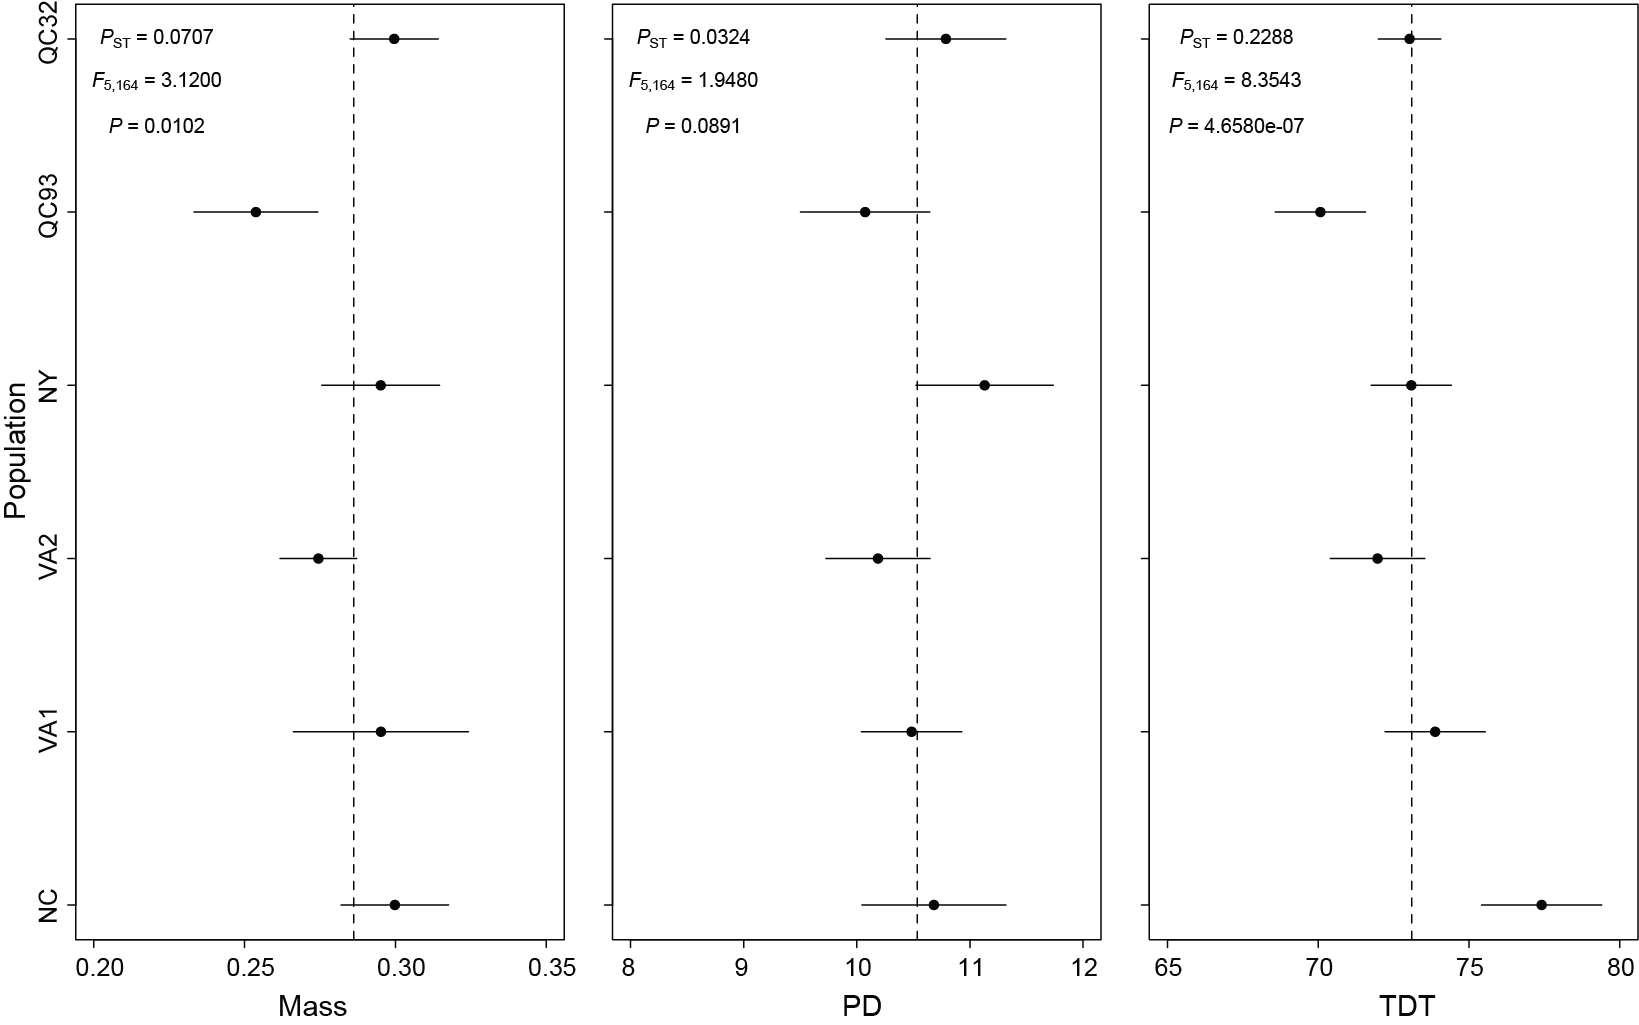
\includegraphics[width=0.9\textwidth]{media/image1.png}
\caption{Mean trait values and their 95\% confidence
intervals (±1.96 × s.e.m) by population for pupal mass (Mass), pupal
duration time (PD), and total development time (TDT). Vertical dashed
lines represent global means for each phenotypic trait.}
\label{fig:trait}
\end{figure}


\begin{figure}
\centering
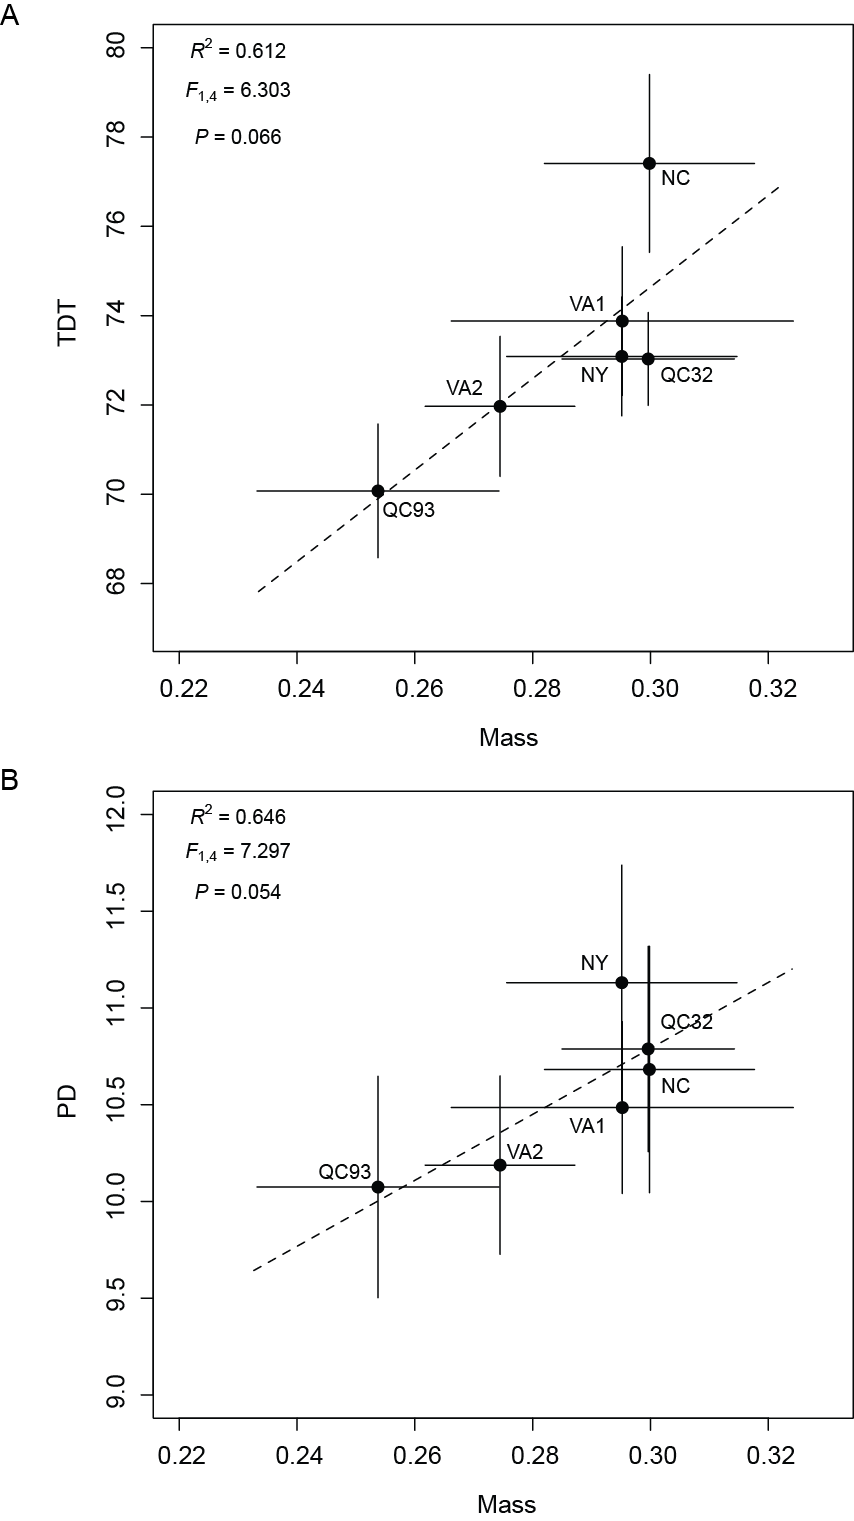
\includegraphics[width=0.6\textwidth]{media/image2.png}
\caption{Correlations among phenotypic trait means by
population that were marginally significant, (A) Pupal mass (Mass)
versus total development time (TDT), (B) Pupal mass (Mass) versus pupal
development time (PD). Statistics in the upper right corner were
generated using a linear model with pupal mass as the predictor of TDT
and PD.}
\label{fig:traitcorr}
\end{figure}
